% Options for packages loaded elsewhere
% Options for packages loaded elsewhere
\PassOptionsToPackage{unicode}{hyperref}
\PassOptionsToPackage{hyphens}{url}
\PassOptionsToPackage{dvipsnames,svgnames,x11names}{xcolor}
%
\documentclass[
  letterpaper,
  DIV=11,
  numbers=noendperiod]{scrartcl}
\usepackage{xcolor}
\usepackage{amsmath,amssymb}
\setcounter{secnumdepth}{-\maxdimen} % remove section numbering
\usepackage{iftex}
\ifPDFTeX
  \usepackage[T1]{fontenc}
  \usepackage[utf8]{inputenc}
  \usepackage{textcomp} % provide euro and other symbols
\else % if luatex or xetex
  \usepackage{unicode-math} % this also loads fontspec
  \defaultfontfeatures{Scale=MatchLowercase}
  \defaultfontfeatures[\rmfamily]{Ligatures=TeX,Scale=1}
\fi
\usepackage{lmodern}
\ifPDFTeX\else
  % xetex/luatex font selection
\fi
% Use upquote if available, for straight quotes in verbatim environments
\IfFileExists{upquote.sty}{\usepackage{upquote}}{}
\IfFileExists{microtype.sty}{% use microtype if available
  \usepackage[]{microtype}
  \UseMicrotypeSet[protrusion]{basicmath} % disable protrusion for tt fonts
}{}
\makeatletter
\@ifundefined{KOMAClassName}{% if non-KOMA class
  \IfFileExists{parskip.sty}{%
    \usepackage{parskip}
  }{% else
    \setlength{\parindent}{0pt}
    \setlength{\parskip}{6pt plus 2pt minus 1pt}}
}{% if KOMA class
  \KOMAoptions{parskip=half}}
\makeatother
% Make \paragraph and \subparagraph free-standing
\makeatletter
\ifx\paragraph\undefined\else
  \let\oldparagraph\paragraph
  \renewcommand{\paragraph}{
    \@ifstar
      \xxxParagraphStar
      \xxxParagraphNoStar
  }
  \newcommand{\xxxParagraphStar}[1]{\oldparagraph*{#1}\mbox{}}
  \newcommand{\xxxParagraphNoStar}[1]{\oldparagraph{#1}\mbox{}}
\fi
\ifx\subparagraph\undefined\else
  \let\oldsubparagraph\subparagraph
  \renewcommand{\subparagraph}{
    \@ifstar
      \xxxSubParagraphStar
      \xxxSubParagraphNoStar
  }
  \newcommand{\xxxSubParagraphStar}[1]{\oldsubparagraph*{#1}\mbox{}}
  \newcommand{\xxxSubParagraphNoStar}[1]{\oldsubparagraph{#1}\mbox{}}
\fi
\makeatother

\usepackage{color}
\usepackage{fancyvrb}
\newcommand{\VerbBar}{|}
\newcommand{\VERB}{\Verb[commandchars=\\\{\}]}
\DefineVerbatimEnvironment{Highlighting}{Verbatim}{commandchars=\\\{\}}
% Add ',fontsize=\small' for more characters per line
\usepackage{framed}
\definecolor{shadecolor}{RGB}{241,243,245}
\newenvironment{Shaded}{\begin{snugshade}}{\end{snugshade}}
\newcommand{\AlertTok}[1]{\textcolor[rgb]{0.68,0.00,0.00}{#1}}
\newcommand{\AnnotationTok}[1]{\textcolor[rgb]{0.37,0.37,0.37}{#1}}
\newcommand{\AttributeTok}[1]{\textcolor[rgb]{0.40,0.45,0.13}{#1}}
\newcommand{\BaseNTok}[1]{\textcolor[rgb]{0.68,0.00,0.00}{#1}}
\newcommand{\BuiltInTok}[1]{\textcolor[rgb]{0.00,0.23,0.31}{#1}}
\newcommand{\CharTok}[1]{\textcolor[rgb]{0.13,0.47,0.30}{#1}}
\newcommand{\CommentTok}[1]{\textcolor[rgb]{0.37,0.37,0.37}{#1}}
\newcommand{\CommentVarTok}[1]{\textcolor[rgb]{0.37,0.37,0.37}{\textit{#1}}}
\newcommand{\ConstantTok}[1]{\textcolor[rgb]{0.56,0.35,0.01}{#1}}
\newcommand{\ControlFlowTok}[1]{\textcolor[rgb]{0.00,0.23,0.31}{\textbf{#1}}}
\newcommand{\DataTypeTok}[1]{\textcolor[rgb]{0.68,0.00,0.00}{#1}}
\newcommand{\DecValTok}[1]{\textcolor[rgb]{0.68,0.00,0.00}{#1}}
\newcommand{\DocumentationTok}[1]{\textcolor[rgb]{0.37,0.37,0.37}{\textit{#1}}}
\newcommand{\ErrorTok}[1]{\textcolor[rgb]{0.68,0.00,0.00}{#1}}
\newcommand{\ExtensionTok}[1]{\textcolor[rgb]{0.00,0.23,0.31}{#1}}
\newcommand{\FloatTok}[1]{\textcolor[rgb]{0.68,0.00,0.00}{#1}}
\newcommand{\FunctionTok}[1]{\textcolor[rgb]{0.28,0.35,0.67}{#1}}
\newcommand{\ImportTok}[1]{\textcolor[rgb]{0.00,0.46,0.62}{#1}}
\newcommand{\InformationTok}[1]{\textcolor[rgb]{0.37,0.37,0.37}{#1}}
\newcommand{\KeywordTok}[1]{\textcolor[rgb]{0.00,0.23,0.31}{\textbf{#1}}}
\newcommand{\NormalTok}[1]{\textcolor[rgb]{0.00,0.23,0.31}{#1}}
\newcommand{\OperatorTok}[1]{\textcolor[rgb]{0.37,0.37,0.37}{#1}}
\newcommand{\OtherTok}[1]{\textcolor[rgb]{0.00,0.23,0.31}{#1}}
\newcommand{\PreprocessorTok}[1]{\textcolor[rgb]{0.68,0.00,0.00}{#1}}
\newcommand{\RegionMarkerTok}[1]{\textcolor[rgb]{0.00,0.23,0.31}{#1}}
\newcommand{\SpecialCharTok}[1]{\textcolor[rgb]{0.37,0.37,0.37}{#1}}
\newcommand{\SpecialStringTok}[1]{\textcolor[rgb]{0.13,0.47,0.30}{#1}}
\newcommand{\StringTok}[1]{\textcolor[rgb]{0.13,0.47,0.30}{#1}}
\newcommand{\VariableTok}[1]{\textcolor[rgb]{0.07,0.07,0.07}{#1}}
\newcommand{\VerbatimStringTok}[1]{\textcolor[rgb]{0.13,0.47,0.30}{#1}}
\newcommand{\WarningTok}[1]{\textcolor[rgb]{0.37,0.37,0.37}{\textit{#1}}}

\usepackage{longtable,booktabs,array}
\usepackage{calc} % for calculating minipage widths
% Correct order of tables after \paragraph or \subparagraph
\usepackage{etoolbox}
\makeatletter
\patchcmd\longtable{\par}{\if@noskipsec\mbox{}\fi\par}{}{}
\makeatother
% Allow footnotes in longtable head/foot
\IfFileExists{footnotehyper.sty}{\usepackage{footnotehyper}}{\usepackage{footnote}}
\makesavenoteenv{longtable}
\usepackage{graphicx}
\makeatletter
\newsavebox\pandoc@box
\newcommand*\pandocbounded[1]{% scales image to fit in text height/width
  \sbox\pandoc@box{#1}%
  \Gscale@div\@tempa{\textheight}{\dimexpr\ht\pandoc@box+\dp\pandoc@box\relax}%
  \Gscale@div\@tempb{\linewidth}{\wd\pandoc@box}%
  \ifdim\@tempb\p@<\@tempa\p@\let\@tempa\@tempb\fi% select the smaller of both
  \ifdim\@tempa\p@<\p@\scalebox{\@tempa}{\usebox\pandoc@box}%
  \else\usebox{\pandoc@box}%
  \fi%
}
% Set default figure placement to htbp
\def\fps@figure{htbp}
\makeatother





\setlength{\emergencystretch}{3em} % prevent overfull lines

\providecommand{\tightlist}{%
  \setlength{\itemsep}{0pt}\setlength{\parskip}{0pt}}



 


\KOMAoption{captions}{tableheading}
\makeatletter
\@ifpackageloaded{caption}{}{\usepackage{caption}}
\AtBeginDocument{%
\ifdefined\contentsname
  \renewcommand*\contentsname{Table of contents}
\else
  \newcommand\contentsname{Table of contents}
\fi
\ifdefined\listfigurename
  \renewcommand*\listfigurename{List of Figures}
\else
  \newcommand\listfigurename{List of Figures}
\fi
\ifdefined\listtablename
  \renewcommand*\listtablename{List of Tables}
\else
  \newcommand\listtablename{List of Tables}
\fi
\ifdefined\figurename
  \renewcommand*\figurename{Figure}
\else
  \newcommand\figurename{Figure}
\fi
\ifdefined\tablename
  \renewcommand*\tablename{Table}
\else
  \newcommand\tablename{Table}
\fi
}
\@ifpackageloaded{float}{}{\usepackage{float}}
\floatstyle{ruled}
\@ifundefined{c@chapter}{\newfloat{codelisting}{h}{lop}}{\newfloat{codelisting}{h}{lop}[chapter]}
\floatname{codelisting}{Listing}
\newcommand*\listoflistings{\listof{codelisting}{List of Listings}}
\makeatother
\makeatletter
\makeatother
\makeatletter
\@ifpackageloaded{caption}{}{\usepackage{caption}}
\@ifpackageloaded{subcaption}{}{\usepackage{subcaption}}
\makeatother
\usepackage{bookmark}
\IfFileExists{xurl.sty}{\usepackage{xurl}}{} % add URL line breaks if available
\urlstyle{same}
\hypersetup{
  pdftitle={Homework 3},
  pdfauthor={Natalie Parker},
  colorlinks=true,
  linkcolor={blue},
  filecolor={Maroon},
  citecolor={Blue},
  urlcolor={Blue},
  pdfcreator={LaTeX via pandoc}}


\title{Homework 3}
\author{Natalie Parker}
\date{2026-05-28}
\begin{document}
\maketitle

\renewcommand*\contentsname{Table of contents}
{
\hypersetup{linkcolor=}
\setcounter{tocdepth}{3}
\tableofcontents
}

\section{Set up}\label{set-up}

\begin{Shaded}
\begin{Highlighting}[]
\FunctionTok{library}\NormalTok{(tidyverse) }\CommentTok{\# general use}
\FunctionTok{library}\NormalTok{(janitor) }\CommentTok{\# cleaning data frames}
\FunctionTok{library}\NormalTok{(here) }\CommentTok{\# file/folder organization}
\FunctionTok{library}\NormalTok{(readxl) }\CommentTok{\# reading .xlsx files}
\FunctionTok{library}\NormalTok{(ggeffects)}
\CommentTok{\# storing kelp data as object "kelp"}
\NormalTok{kelp }\OtherTok{\textless{}{-}} \FunctionTok{read.csv}\NormalTok{(}\FunctionTok{here}\NormalTok{(}\StringTok{"data"}\NormalTok{, }\StringTok{"temp{-}kelp.csv"}\NormalTok{))}
\CommentTok{\# creating new object that fits a linear model to the data}
\NormalTok{kelp\_model }\OtherTok{\textless{}{-}} \FunctionTok{lm}\NormalTok{(}
\NormalTok{  kelp\_elong }\SpecialCharTok{\textasciitilde{}}\NormalTok{ temp\_c, }
  \AttributeTok{data =}\NormalTok{ kelp)}
\CommentTok{\# storing and cleaning personal data as object "personal\_clean"}
\NormalTok{personal\_clean }\OtherTok{\textless{}{-}} \FunctionTok{read\_csv}\NormalTok{(}
  \FunctionTok{here}\NormalTok{(}\StringTok{"data"}\NormalTok{, }\StringTok{"ENVS 193DS{-} Personal Data {-} Sheet1.csv"}\NormalTok{), }
  \CommentTok{\# skipping the first 2 messed up rows}
  \AttributeTok{skip =} \DecValTok{2}\NormalTok{) }\SpecialCharTok{|\textgreater{}} 
  \CommentTok{\# dropping the first empty column}
  \FunctionTok{select}\NormalTok{(}\SpecialCharTok{{-}}\DecValTok{1}\NormalTok{) }\SpecialCharTok{|\textgreater{}} 
  \CommentTok{\# cleaning the names}
  \FunctionTok{clean\_names}\NormalTok{() }\SpecialCharTok{|\textgreater{}} 
 \CommentTok{\# converting sleep to a graphable value}
  \FunctionTok{mutate}\NormalTok{(}
    \AttributeTok{sleep\_hours =} 
      \FunctionTok{hour}\NormalTok{(}\FunctionTok{hms}\NormalTok{(amount\_of\_sleep)) }\SpecialCharTok{+}\NormalTok{ (}\FunctionTok{minute}\NormalTok{(}\FunctionTok{hms}\NormalTok{(amount\_of\_sleep)) }\SpecialCharTok{/} \DecValTok{60}\NormalTok{),}
    \CommentTok{\# converting the columns of "date", "caffeine", and "satisfaction" to numbers and dates}
    \AttributeTok{date =} \FunctionTok{as.Date}\NormalTok{(date, }\AttributeTok{format =} \StringTok{"\%m/\%d/\%Y"}\NormalTok{),}
    \AttributeTok{caffeine =} \FunctionTok{as.numeric}\NormalTok{(caffeine),}
    \AttributeTok{satisfaction =} \FunctionTok{as.numeric}\NormalTok{(satisfaction))}
\end{Highlighting}
\end{Shaded}

\section{Problem 1}\label{problem-1}

\subsection{1a.}\label{a.}

The appropriate tests would be the Pearson's correlation and linear
regression to determine the strength of the relationship between giant
kelp frond elongation rate and temperature. Pearson's correlation
measures the strength and the direction between the two variables.
Linear regression aims to describe a linear relationship between the
variables while being able to describe strength as well.

\subsection{1b.}\label{b.}

\begin{Shaded}
\begin{Highlighting}[]
\CommentTok{\# creating new object called kelp\_preds}
\NormalTok{kelp\_preds }\OtherTok{\textless{}{-}} \FunctionTok{ggpredict}\NormalTok{(}
\NormalTok{  kelp\_model, }
  \AttributeTok{terms =} \StringTok{"temp\_c"}\NormalTok{)}
\CommentTok{\# base layer: ggplot with kelp data}
\FunctionTok{ggplot}\NormalTok{(}\AttributeTok{data =}\NormalTok{ kelp, }
       \FunctionTok{aes}\NormalTok{ (}\AttributeTok{x =}\NormalTok{ temp\_c, }\CommentTok{\# x{-}axis is sea temp}
            \AttributeTok{y =}\NormalTok{ kelp\_elong)) }\SpecialCharTok{+} \CommentTok{\# y{-}axis is kelp elongation rate}
  \CommentTok{\# first layer: geom\_point to show underlying data}
  \FunctionTok{geom\_point}\NormalTok{(}\AttributeTok{fill =} \StringTok{"\#1f78b4"}\NormalTok{, }\CommentTok{\# changing the color and size}
             \AttributeTok{size =} \DecValTok{4}\NormalTok{, }
             \AttributeTok{stroke =} \DecValTok{1}\NormalTok{,}
             \AttributeTok{shape =} \DecValTok{21}\NormalTok{) }\SpecialCharTok{+} 
 \CommentTok{\# second layer: ribbon representing confidence interval}
 \CommentTok{\# using predictions data frame}
 \FunctionTok{geom\_ribbon}\NormalTok{(}\AttributeTok{data =}\NormalTok{ kelp\_preds,}
             \FunctionTok{aes}\NormalTok{(}\AttributeTok{x =}\NormalTok{ x,}
                 \AttributeTok{y =}\NormalTok{ predicted, }
                 \AttributeTok{ymin =}\NormalTok{ conf.low,}
                 \AttributeTok{ymax =}\NormalTok{ conf.high),}
             \AttributeTok{alpha =} \FloatTok{0.1}\NormalTok{) }\SpecialCharTok{+}
  \CommentTok{\# third layer: line representing model predictions}
  \FunctionTok{geom\_line}\NormalTok{(}\AttributeTok{data =}\NormalTok{ kelp\_preds,}
            \FunctionTok{aes}\NormalTok{(}\AttributeTok{x =}\NormalTok{ x,}
                \AttributeTok{y =}\NormalTok{ predicted),}
            \AttributeTok{linewidth =} \DecValTok{1}\NormalTok{)}\SpecialCharTok{+}
   \FunctionTok{labs}\NormalTok{ ( }\AttributeTok{x=} \StringTok{"Average Ocean Temperature (°C)"}\NormalTok{,}
         \AttributeTok{y =} \FunctionTok{bquote}\NormalTok{(Frond}\SpecialCharTok{\textasciitilde{}}\NormalTok{Elongation}\SpecialCharTok{\textasciitilde{}}\NormalTok{Rate}\SpecialCharTok{\textasciitilde{}}\NormalTok{(cm}\SpecialCharTok{\textasciitilde{}}\NormalTok{day}\SpecialCharTok{\^{}{-}}\DecValTok{1}\NormalTok{)),}
                    \AttributeTok{title =} \StringTok{"Giant Kelp Elongation Rate vs. Ocean Temperature"}\NormalTok{) }\SpecialCharTok{+}
  \CommentTok{\# changing the theme}
  \FunctionTok{theme\_minimal}\NormalTok{() }\SpecialCharTok{+}
  \CommentTok{\# customizing the look of the titles!}
  \FunctionTok{theme}\NormalTok{(}\AttributeTok{plot.title =} \FunctionTok{element\_text}\NormalTok{(}\AttributeTok{face =} \StringTok{"bold"}\NormalTok{,}
                                  \AttributeTok{size =} \DecValTok{14}\NormalTok{, }
                                  \AttributeTok{hjust =} \FloatTok{0.5}\NormalTok{),}
        \AttributeTok{axis.title =} \FunctionTok{element\_text}\NormalTok{(}\AttributeTok{face =} \StringTok{"plain"}\NormalTok{,}
                                  \AttributeTok{size =} \DecValTok{11}\NormalTok{))}
\end{Highlighting}
\end{Shaded}

\pandocbounded{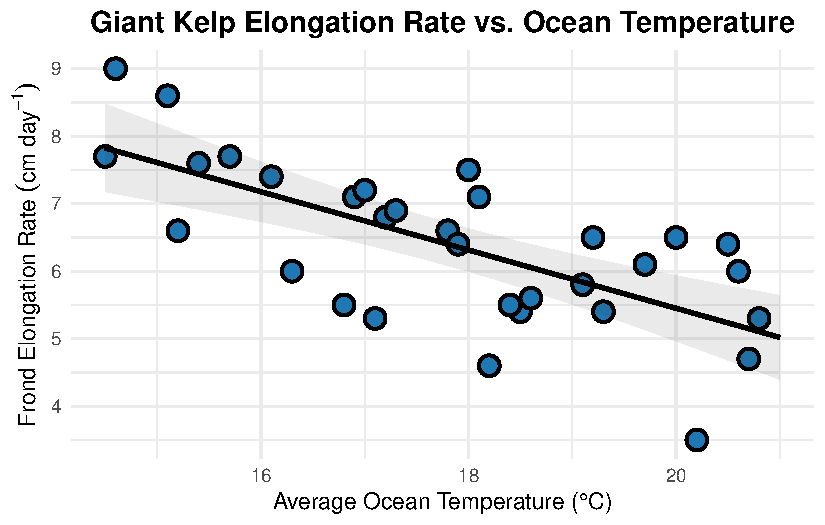
\includegraphics[keepaspectratio]{homework-qurtodoc_files/figure-pdf/visualization-of-temp-and-kelp-1.pdf}}

\subsection{1c.}\label{c.}

\subsubsection{Checking assumptions}\label{checking-assumptions}

\begin{Shaded}
\begin{Highlighting}[]
\CommentTok{\# base R residuals}
\FunctionTok{par}\NormalTok{(}\AttributeTok{mfrow =} \FunctionTok{c}\NormalTok{(}\DecValTok{2}\NormalTok{,}\DecValTok{2}\NormalTok{))}
\FunctionTok{plot}\NormalTok{(kelp\_model)}
\end{Highlighting}
\end{Shaded}

\pandocbounded{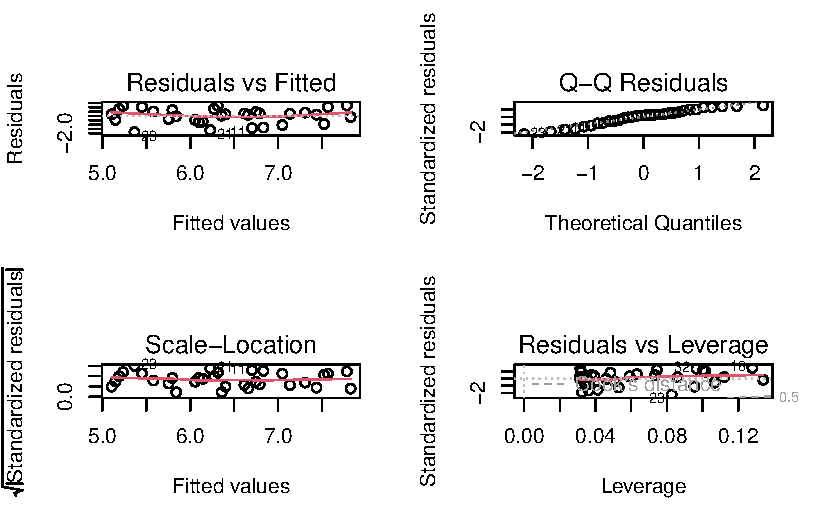
\includegraphics[keepaspectratio]{homework-qurtodoc_files/figure-pdf/diagnostic-plots-to-check-assumptions-1.pdf}}

When thinking about the relationship between ocean temperature and kelp
elongation, it would make sense for there to be a linear relationship.
We can see this in the residuals vs.~fitted plot and the plotted data.
We can assume independent errors due to the independent observations and
data collection methods. The residual vs.~fitted and scale location
plots both show us the homoscedasticity of errors. The plots show that
the data is homoscedastic because of the decently straight trend line.
Looking at the QQ plot seen in residual plots, the data seems to be
normally distributed. It roughly follows the straight line with
variations that are normal to see in real data.

I think I did ok checking the assumptions. It's hard because making the
decision is subjective, but generally most math isn't, and making the
``wrong'' choice can have big impacts. The QQ plot was hardest to assess
due to the slight curve seen in it.

\subsubsection{Running test}\label{running-test}

\begin{Shaded}
\begin{Highlighting}[]
\CommentTok{\# showing the output of linear regression}
\FunctionTok{summary}\NormalTok{(kelp\_model)}
\end{Highlighting}
\end{Shaded}

\begin{verbatim}

Call:
lm(formula = kelp_elong ~ temp_c, data = kelp)

Residuals:
    Min      1Q  Median      3Q     Max 
-1.8643 -0.5017  0.1790  0.5659  1.2177 

Coefficients:
            Estimate Std. Error t value Pr(>|t|)    
(Intercept) 14.08645    1.49219   9.440 1.72e-10 ***
temp_c      -0.43179    0.08321  -5.189 1.37e-05 ***
---
Signif. codes:  0 '***' 0.001 '**' 0.01 '*' 0.05 '.' 0.1 ' ' 1

Residual standard error: 0.8665 on 30 degrees of freedom
Multiple R-squared:  0.473, Adjusted R-squared:  0.4554 
F-statistic: 26.93 on 1 and 30 DF,  p-value: 1.366e-05
\end{verbatim}

\subsection{1d.}\label{d.}

To evaluate the strength of the relationship between temperature and
giant kelp frond elongation rate, I used an F test from a linear
regression model. I used the linear regression model because the data
met the assumptions for the model and the goal was to test the strength
of the relationship of the variables. A linear model is great for
testing strength and relationship. I used the f-test because it's
traditional to get the output for an F-test when creating a linear
model.

We reject the null hypothesis, so the elongation rate of giant kelp
decreased as the average ocean temperature increased (linear regression,
F(30,1) = 26.93, R\textsuperscript{2} = 0.473, p\textless{} 0.001,
\(\alpha\) = 0.05)

Based on Model predictions, for each unit 1 increase in ocean
temperature, we expect an decrease of 0.43 \(\pm\) 0.08 (SE) cm
day\textsuperscript{-1}.

\subsection{1e.}\label{e.}

This test used the data collected from kelp in varying ocean
temperatures to understand how increasing ocean temperature can affect
giant kelp growth. From performing a F test for significance and a
linear regression model for strength of the relationship, we were able
to understand that when average ocean temp increases, we see a decrease
in giant kelp elongation. This means that for giant kelp to be at their
healthiest, ocean temperatures cannot continue to increase.

\subsection{1f.}\label{f.}

\begin{Shaded}
\begin{Highlighting}[]
\CommentTok{\# creating new object for pearson\textquotesingle{}s test from kelp data and running pearson\textquotesingle{}s test}
\NormalTok{kelp\_corr }\OtherTok{\textless{}{-}} \FunctionTok{cor.test}\NormalTok{(kelp}\SpecialCharTok{$}\NormalTok{temp\_c, }
\NormalTok{                      kelp}\SpecialCharTok{$}\NormalTok{kelp\_elong, }
                      \AttributeTok{method =} \StringTok{"pearson"}\NormalTok{)}
\CommentTok{\# displaying test output}
\NormalTok{kelp\_corr}
\end{Highlighting}
\end{Shaded}

\begin{verbatim}

    Pearson's product-moment correlation

data:  kelp$temp_c and kelp$kelp_elong
t = -5.189, df = 30, p-value = 1.366e-05
alternative hypothesis: true correlation is not equal to 0
95 percent confidence interval:
 -0.8359665 -0.4460157
sample estimates:
       cor 
-0.6877489 
\end{verbatim}

Both tests would have lead to the exact same decision of rejecting the
null hypothesis because they have identical t-values of -5.189, p-values
of 1.366e-05, and the same significance level of 0.05. They also come to
the same conclusion for correlation and strength because of they have to
same regression coefficient (-0.688), which is equal to the R squared
value of 0.473 when squared. They both show a strong negative
correlation between increase in temp and kelp elongation.

\section{Problem 2}\label{problem-2}

\subsection{2a.}\label{a.-1}

\begin{Shaded}
\begin{Highlighting}[]
\CommentTok{\# base layer: ggplot}
\FunctionTok{ggplot}\NormalTok{(}\AttributeTok{data =}\NormalTok{ personal\_clean,}
       \CommentTok{\# x{-}axis is length of wo, y{-}axis is satisfaction}
       \FunctionTok{aes}\NormalTok{(}\AttributeTok{x =}\NormalTok{ length\_of\_wo,}
           \AttributeTok{y =}\NormalTok{ satisfaction)) }\SpecialCharTok{+}
  \CommentTok{\# first layer: point, points with a custom color}
  \FunctionTok{geom\_point}\NormalTok{(}\AttributeTok{color =} \StringTok{"cyan4"}\NormalTok{, }\AttributeTok{size =} \DecValTok{4}\NormalTok{, }\AttributeTok{alpha =} \FloatTok{0.8}\NormalTok{) }\SpecialCharTok{+}
  \CommentTok{\# clean theme}
  \FunctionTok{theme\_bw}\NormalTok{() }\SpecialCharTok{+}
  \CommentTok{\# removing the excess grid marks}
  \FunctionTok{theme}\NormalTok{(}\AttributeTok{panel.grid.minor =} \FunctionTok{element\_blank}\NormalTok{())}\SpecialCharTok{+}
  \CommentTok{\# labels and title}
  \FunctionTok{labs}\NormalTok{(}
    \AttributeTok{x =} \StringTok{"Length of Workout (hours)"}\NormalTok{,}
    \AttributeTok{y =} \StringTok{"Satisfaction Score (1{-}5)"}\NormalTok{,}
    \AttributeTok{title =} \StringTok{"Workout Length in Relation to Satisfaction"}\NormalTok{,}
    \AttributeTok{subtitle =} \StringTok{"05/27/26"}\NormalTok{)}
\end{Highlighting}
\end{Shaded}

\pandocbounded{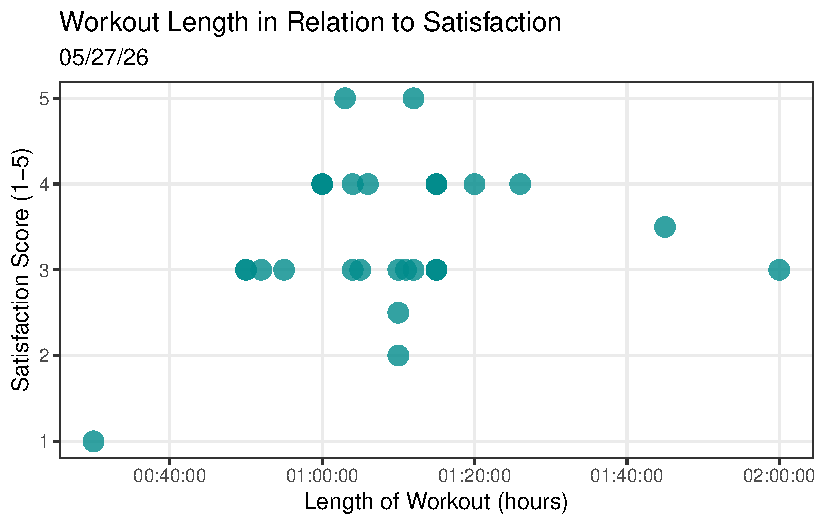
\includegraphics[keepaspectratio]{homework-qurtodoc_files/figure-pdf/original-length-vs.-satisfaction-1.pdf}}

\subsection{2b.}\label{b.-1}

Figure 2. Length of workout doesn't influence satisfaction. Data
collected from workouts taken place in the time period 4-20-2026 to
5-27-2026 (Data accessed 05-28-2026). Teal points represent individual
observations of length of workout (hours) (total n = 30) plotted against
satisfaction with workout (1-5).

\begin{Shaded}
\begin{Highlighting}[]
\NormalTok{workout\_model }\OtherTok{\textless{}{-}} \FunctionTok{lm}\NormalTok{(satisfaction }\SpecialCharTok{\textasciitilde{}}\NormalTok{ sleep\_hours, }\AttributeTok{data =}\NormalTok{ personal\_clean)}
\NormalTok{personal\_preds }\OtherTok{\textless{}{-}} \FunctionTok{ggpredict}\NormalTok{(workout\_model, }
                            \AttributeTok{terms =} \StringTok{"sleep\_hours"}\NormalTok{)}
\CommentTok{\#base layer: ggplot }
\FunctionTok{ggplot}\NormalTok{() }\SpecialCharTok{+}
  \CommentTok{\# second layer: geom\_point to show underlying data with personal\_clean data}
  \FunctionTok{geom\_point}\NormalTok{( }\AttributeTok{data =}\NormalTok{ personal\_clean, }
       \FunctionTok{aes}\NormalTok{(}\AttributeTok{x =}\NormalTok{ sleep\_hours, }
       \AttributeTok{y =}\NormalTok{ satisfaction), }
       \AttributeTok{fill =} \StringTok{"\#ac88ff"}\NormalTok{,}
       \AttributeTok{size =} \DecValTok{4}\NormalTok{,}
       \AttributeTok{stroke =} \DecValTok{1}\NormalTok{,}
       \AttributeTok{shape =} \DecValTok{21}\NormalTok{) }\SpecialCharTok{+}
  \CommentTok{\# third layer: geom\_ribbon to show CI}
 \CommentTok{\# using predictions data frame}
 \FunctionTok{geom\_ribbon}\NormalTok{(}\AttributeTok{data =}\NormalTok{ personal\_preds,}
             \FunctionTok{aes}\NormalTok{(}\AttributeTok{x =}\NormalTok{ x,}
                 \AttributeTok{y =}\NormalTok{ predicted, }
                 \AttributeTok{ymin =}\NormalTok{ conf.low,}
                 \AttributeTok{ymax =}\NormalTok{ conf.high),}
             \AttributeTok{fill =} \StringTok{"\#00bdd0"}\NormalTok{,}
             \AttributeTok{alpha =} \FloatTok{0.1}\NormalTok{) }\SpecialCharTok{+}
  \CommentTok{\# third layer: line representing model predictions}
  \FunctionTok{geom\_line}\NormalTok{(}\AttributeTok{data =}\NormalTok{ personal\_preds,}
            \FunctionTok{aes}\NormalTok{(}\AttributeTok{x =}\NormalTok{ x,}
                \AttributeTok{y =}\NormalTok{ predicted),}
            \AttributeTok{color =} \StringTok{"\#00bdd0"}\NormalTok{,}
            \AttributeTok{linewidth =} \DecValTok{1}\NormalTok{) }\SpecialCharTok{+}
  \CommentTok{\# adding axes titles and titles!}
  \FunctionTok{labs}\NormalTok{(}
    \AttributeTok{x =} \StringTok{"Amount of Sleep (Hours)"}\NormalTok{,}
    \AttributeTok{y =} \StringTok{"Workout Satisfaction Score (1{-}5)"}\NormalTok{,}
    \AttributeTok{title =} \StringTok{"Workout Satisfaction Predicted by Sleep Duration"}\NormalTok{,}
    \AttributeTok{subtitle =} \StringTok{"05/27/26"}\NormalTok{) }\SpecialCharTok{+}
  \CommentTok{\# changing theme}
  \FunctionTok{theme\_classic}\NormalTok{() }\SpecialCharTok{+}
  \CommentTok{\# removing grid lines, bolding title, and changing axes text}
  \FunctionTok{theme}\NormalTok{(}
    \AttributeTok{panel.grid.major =} \FunctionTok{element\_blank}\NormalTok{(),}
    \AttributeTok{panel.grid.minor =} \FunctionTok{element\_blank}\NormalTok{(),}
    \AttributeTok{plot.title =} \FunctionTok{element\_text}\NormalTok{(}\AttributeTok{face =} \StringTok{"bold"}\NormalTok{, }\AttributeTok{size =} \DecValTok{13}\NormalTok{, }\AttributeTok{hjust =} \FloatTok{0.5}\NormalTok{),}
    \AttributeTok{axis.title =} \FunctionTok{element\_text}\NormalTok{(}\AttributeTok{face =} \StringTok{"plain"}\NormalTok{, }\AttributeTok{size =} \DecValTok{11}\NormalTok{))}
\end{Highlighting}
\end{Shaded}

\pandocbounded{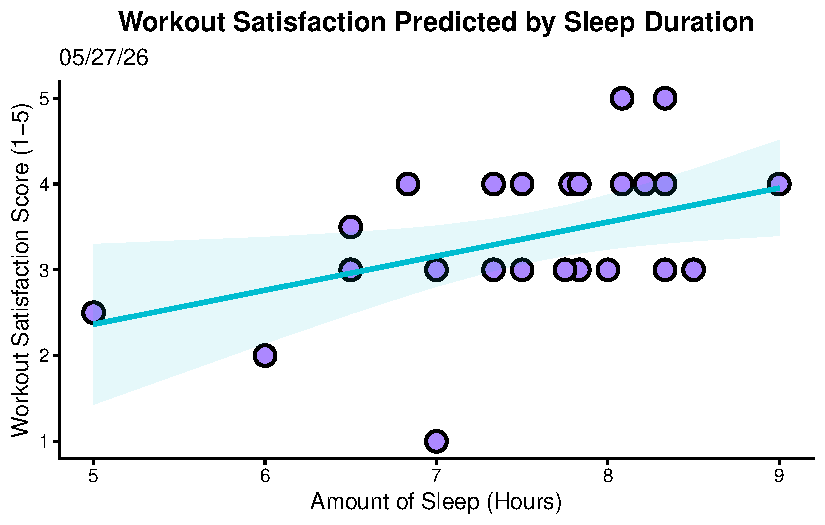
\includegraphics[keepaspectratio]{homework-qurtodoc_files/figure-pdf/new-satisfaction-vs.-sleep-1.pdf}}

\subsection{2b.}\label{b.-2}

Figure 3. Less sleep is associated with lower workout satisfaction. Data
collected from workouts taken place in the time period 4-20-2026 to
5-27-2026 (Data accessed 05-28-2026). Purple points represent individual
observations of amount fo sleep (hours) (total n = 30) plotted against
workout satisfaction score (1-5). Teal, thin line represent the linear
regression model prediction for workout satisfaction given amount of
sleep. Thick, transparent, teal stripe represents 95\% confidence
interval of linear regression model.

\section{Problem 3}\label{problem-3}

\subsection{3a.}\label{a.-2}

An affective visualization for my personal data could be done in a
variety of ways. My idea is to use circles to represent each workout.
The size of the circle is based on sleep, the color is based on
satisfaction, the type of workout would be some pattern or symbol on the
circle, and a handful of other features for the other variables. This
would work for my data because it has the ability to have lots of
different features, and my data collection has many different variables.

\subsection{3b.}\label{b.-3}

\subsection{3c.}\label{c.-1}

\subsection{3d.}\label{d.-1}

\subsection{3e.}\label{e.-1}

\section{Problem 4}\label{problem-4}

\subsection{4a.}\label{a.-3}

The test for this paper is Mann- Whitney U. This test addresses the main
question of ``if the lead contamination in neighborhoods in Huntington
Park are higher than other places in LA?'' by showing a potential
significant difference using a p-value (p\textless0.01). If there was a
significant difference seen, that means that the lead contamination in
Huntington Park would be higher than the surrounding areas. This test
works for this because they're independent and not normally distributed.
\pandocbounded{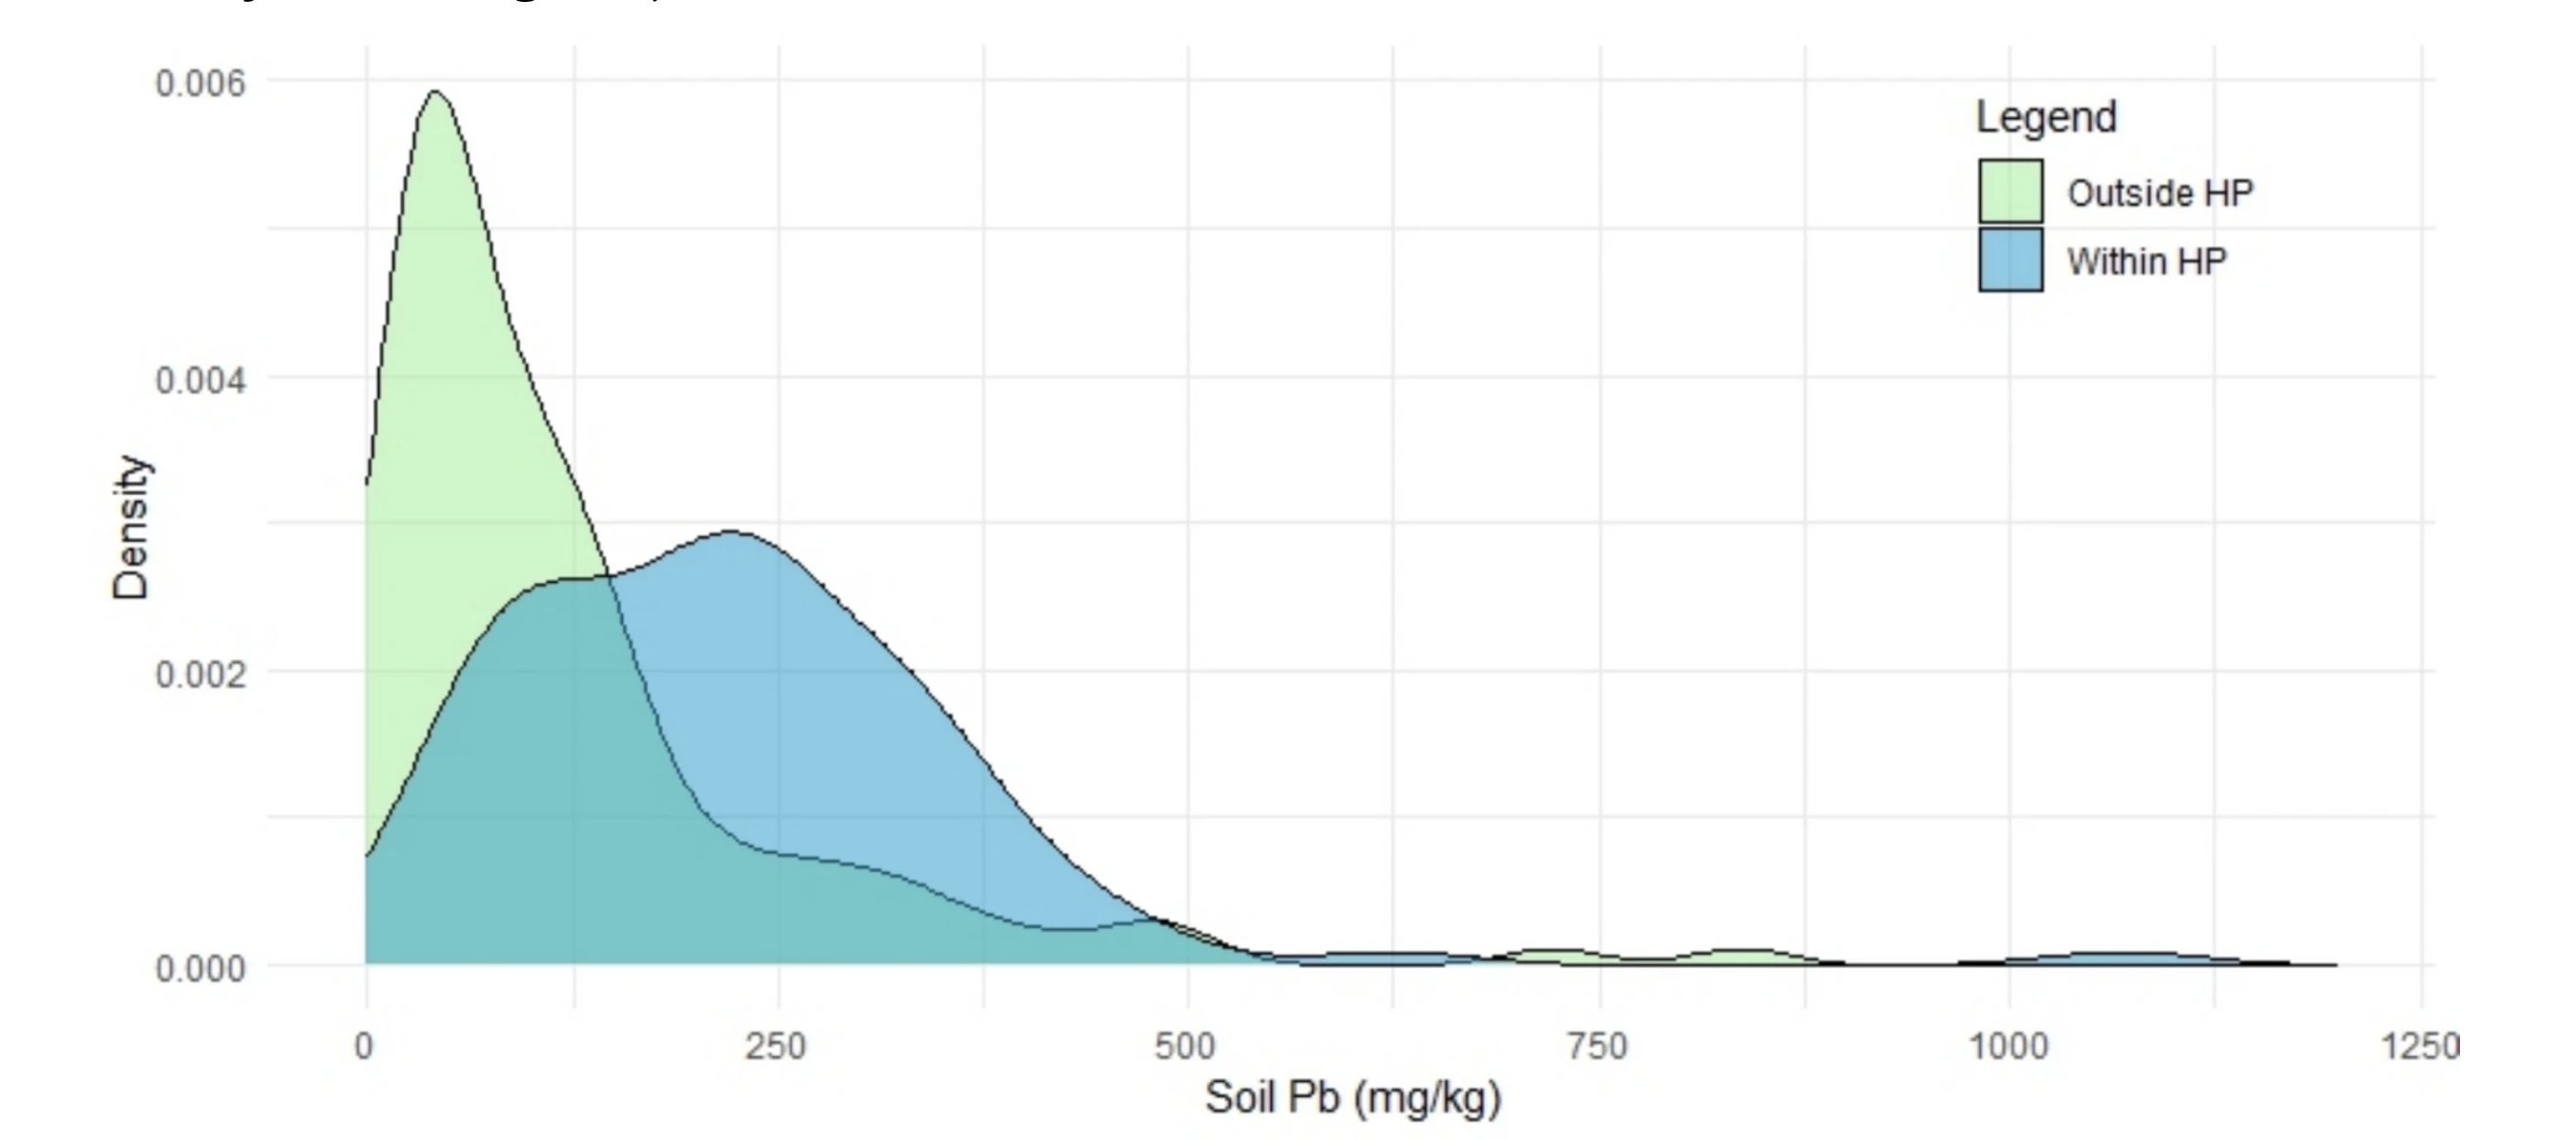
\includegraphics[keepaspectratio]{screenshot.png}}




\end{document}
